\chapter{Literature review}
\label{chapter:literature-review}

To enhance the functionality of vulnerability management in \ac{SCA} Tool, it is essential to conduct a thorough review of existing research in vulnerability classification and remediation. This chapter provides an overview of current models, tools, and approaches in the field. The insights gained serve as the foundation for the development of a multidimensional classification and remediation model, as well as algorithms to assess, prioritize, and recommend remediation actions for vulnerabilities in software projects. The findings from this literature review directly inform the multidimensional model developed in chapter~\ref{chapter:multidimensional-vulnerability-classification}.

\section{Existing Vulnerability Identification and Classification Models}
\label{sec:existing-vulnerability-identification}

Vulnerability classification models provide structured methods for assessing and prioritizing security vulnerabilities based on factors such as severity, exploitability, and potential impact.

Given that the vulnerability management system in \ac{SCA} Tool retrieves vulnerability information from the \ac{OSV} Database, which heavily relies on the \ac{CVE} system for uniquely identifying vulnerabilities, it is essential to include \ac{CVE} in this discussion. \ac{CVE} acts as the foundational identification system that standardizes the naming of vulnerabilities, enabling consistent referencing across databases, tools, and classification models. Although \ac{CVE} itself does not classify vulnerabilities, it provides the standardized identifiers necessary for databases and tools to organize and retrieve vulnerability information consistently \autocite{mitre_corporation_overview_2024}.

Models such as \ac{CVSS} and \ac{EPSS} offer standardized approaches to vulnerability classification. Classifications generated by these models are typically stored in vulnerability databases, linked by their respective \ac{CVE} identifiers. Tools and systems implementing these classification models subsequently access these databases to evaluate vulnerability severity and exploitability.

\ac{CVSS} has been selected for its structured scoring system that assesses vulnerabilities according to their severity. However, recognizing the limitations of \ac{CVSS} (see section \ref{subsec:common-vulnerability-scoring-system}), \ac{EPSS} is incorporated to enrich prioritization through dynamic threat intelligence. Additionally, \ac{SSVC} is integrated due to its consideration of stakeholder-specific factors. Using tailored decision trees, \ac{SSVC} guides context-sensitive prioritization and remediation decisions, helping organizations choose appropriate responses such as patching, monitoring, or deprioritizing vulnerabilities, based on their operational contexts and resources.

Other models, such as \ac{CWE}\footnote{\url{https://cwe.mitre.org/}} and \ac{CAPEC}\footnote{\url{https://capec.mitre.org/}}, primarily focus on categorizing software weaknesses and attack patterns rather than directly classifying vulnerabilities. While these models are valuable in broader security contexts, they are less directly applicable to the specific goals of vulnerability classification and remediation within \ac{SCA} tools.

In summary, the vulnerability management system in \ac{SCA} Tool builds upon the foundational identification provided by \ac{CVE}, using it to retrieve comprehensive vulnerability details from relevant databases, which are then leveraged by classification models to support effective vulnerability assessment and remediation. The following sections present these classification models and their underlying concepts in greater detail.

\subsection{Common Vulnerabilities and Exposures}
\label{subsec:common-vulnerabilities-exposures}

The \ac{CVE} system provides a well-established and standardized framework for uniquely identifying and referencing publicly disclosed cybersecurity vulnerabilities. It is maintained by the \ac{MITRE} and funded by the \ac{CISA}. Each vulnerability in the \ac{CVE} system is assigned a unique identifier, such as \texttt{CVE-2024-12345}, which acts as a universal reference point for tools, databases, and discussions related to cybersecurity. The \ac{CVE} entries contain basic metadata, such as the vulnerability description, affected products, and references to further details. However, \ac{CVE} itself does not include technical details, exploit code, or remediation instructions. Instead, it serves as a reference system that links to external sources for further information.

The structure of a \ac{CVE} identifier follows the format \texttt{CVE-YYYY-NNNNN}, where:
\begin{itemize}
    \item \textbf{YYYY (e.g., 2024)}: Indicates the year in which the CVE-ID was assigned or reserved. This helps provide a temporal context for when the vulnerability became publicly known or cataloged.
    \item \textbf{NNNNN (e.g., 12345)}: Represents a unique, sequential number that identifies the vulnerability within the specified year. This number is assigned by the \ac{CVE} system to ensure uniqueness.
\end{itemize}

For example, in the identifier \texttt{CVE-2024-12345}:
\begin{itemize}
    \item \texttt{2024} indicates that the CVE-ID was assigned or cataloged in the year 2024.
    \item \texttt{12345} is the specific, unique number that distinguishes this vulnerability from others cataloged in the same year.
\end{itemize}

The primary objective of \ac{CVE} is to improve the coordination and sharing of vulnerability information across different organizations, tools, and platforms. By providing a consistent and unique identifier for each vulnerability, \ac{CVE} enables organizations to align their vulnerability management processes, ensuring that the same vulnerability is referenced accurately in security tools, advisories, and incident response processes.

While \ac{CVE} is not a classification or scoring system, it enables security tools and vulnerability management systems to retrieve vulnerability data, such as \ac{CVSS} and \ac{EPSS}, from databases by providing a standardized identification mechanism \autocite{mitre_corporation_overview_2024}. 
\\
In the implementation (see section~\ref{subsec:caching-repository}), the \ac{CVE} system acts as the primary identifier used to retrieve corresponding vulnerability details from external databases such as \ac{NVD} and \texttt{first.org}'s \ac{EPSS}, facilitating standardized data integration into the vulnerability management workflow.

\subsection{Common Vulnerability Scoring System}
\label{subsec:common-vulnerability-scoring-system}

The \ac{CVSS} provides a method to capture the essential characteristics of a vulnerability, reflecting its severity to help organizations assess and prioritize their vulnerability management processes. However, the scoring algorithm lacks formal and empirical justification, and its creators caution against using \ac{CVSS} as a risk score, though some compliance bodies, such as the U.S. government and the global payment card industry, explicitly recommend this misuse \autocite{spring_time_2021}.

The \ac{CVSS} scoring framework (Version 3.1, currently the most widely adopted version)\footnote{\url{https://vulncheck.com/blog/common-vulnerability-scoring-system}} is structured into three metric groups: Base, Temporal, and Environmental. Each group contributes uniquely to the final score \autocite{first_cvss_2025}:

\begin{itemize} 
    \item \textbf{Base Metrics}: Capture characteristics of a vulnerability that remain constant over time and across environments, such as access complexity, authentication requirements, and impacts on confidentiality, integrity, and availability. 
    \item \textbf{Temporal Metrics}: Reflect aspects that can change over time, like the availability of exploit code or patches, which adjust the base score to represent the current level of exploitability. 
    \item \textbf{Environmental Metrics}: Allow organizations to adjust the score based on their specific context, incorporating factors like potential collateral damage and the prevalence of affected systems, providing a customized risk assessment more reflective of the organization's environment. 
\end{itemize}

Despite its structured approach, the \ac{CVSS} scoring system faces criticism for several significant limitations. The process of converting qualitative evaluations into a numerical score between 0 and 10 has been critiqued for assigning numerical values to ordinal data without sufficient empirical justification. This methodology can produce inconsistent and sometimes misleading scores, as it overlooks important contextual factors. Additionally, studies have shown high variability in \ac{CVSS} scoring even among experienced security professionals, with score discrepancies of 2–4 points being common. Such discrepancies are substantial, given that four points span the entire "high" severity range, highlighting a lack of precision in the system \autocite{spring_time_2021}.

\subsubsection{Evolution of CVSS Versions}
\label{subsubsec:cvss-versions}

According to \textcite{balbix_inc_cvss_2020}, the \ac{CVSS} has evolved over time to address the limitations of earlier versions. Each new version introduces improvements to enhance the accuracy and usability of vulnerability assessments.

\paragraph{CVSS Version 1}
\label{par:cvss-v1}

The first version of \ac{CVSS} was the initial attempt to standardize vulnerability scoring but lacked the necessary granularity and flexibility. It did not adequately represent factors like attack complexity or impacts on integrity and availability, leading to limited adoption.

\paragraph{CVSS Version 2}
\label{par:cvss-v2}

The second version improved upon the first version by introducing more detailed metrics and a better framework for assessing vulnerabilities. It considered aspects like access vectors, access complexity, and authentication requirements. However, it still faced challenges in accurately representing modern vulnerabilities, particularly regarding the complexity of required privileges and user interactions.

\paragraph{CVSS Version 3}
\label{par:cvss-v3}

The third generation further refined the scoring system by adding new metrics and modifying existing ones for a more precise and context-aware evaluation. It offers detailed considerations of the attack vector and includes metrics for privileges required and user interaction. These improvements help organizations better prioritize risks and develop effective security strategies.

\paragraph{CVSS Version 3.1}
\label{par:cvss-v3_1}

\ac{CVSS} 3.1 builds on the enhancements introduced in Version 3 by refining certain metrics and clarifying guidelines to achieve more accurate and consistent vulnerability assessments. It also standardizes terminology and scoring interpretations, which helps ensure comparability across various systems and tools \autocite{first_cvss_2024}. Additionally, as confirmed by current security sources, Version 3.1 remains the officially recognized standard today, enabling organizations to effectively prioritize and address risks.\footnote{\url{https://vulncheck.com/blog/common-vulnerability-scoring-system}}

\paragraph{CVSS Version 4}
\label{par:cvss-v4}

The latest version, \ac{CVSS} Version 4.0, has been proposed to address ongoing criticisms but, at the time of writing, has not yet been widely adopted or fully standardized. The most recent revision of its documentation (V1.2, released June 18, 2024) reflects ongoing adjustments and clarifications. Organizations often hesitate to transition to a new major version until it gains broad industry acceptance. Consequently, \ac{CVSS} Version 3.1 remains the dominant standard for vulnerability assessment \autocite{first_cvss_2024_v4}.

\ac{CVSS} helps assess technical severity, but it does not fully account for security risk, leaving room for improvement. Particularly notable is the documented scoring inconsistency of 2–4 points observed among experienced security practitioners \autocite{spring_time_2021}. 

This variability can lead to misaligned remediation efforts, emphasizing the need for complementary metrics. To address these limitations, the multidimensional classification model proposed in this thesis (see section~\ref{sec:multi-dimensional-classification}) integrates exploitability indicators such as \ac{EPSS}, thus achieving a more consistent and risk-oriented prioritization.

\subsection{Exploit Prediction Scoring System}
\label{subsec:epss-theoretical-basis}

The \ac{EPSS} is an open, data-driven framework for assessing the threat posed by software vulnerabilities. It aims to quantify the probability that a vulnerability will be exploited in the wild within the first 12 months after its public disclosure. Unlike traditional methods that often rely on subjective expert opinions or severity scores like the \ac{CVSS}, \ac{EPSS} utilizes objective, publicly available data and machine learning to make accurate predictions.

\ac{EPSS} employs a logistic regression model that is simple to implement and interpret. By reducing the number of required input variables and focusing on publicly accessible data sources, it offers high predictive accuracy regarding the likelihood of exploitation. Key factors in the model include:

\begin{itemize}
    \item \textbf{Availability of Exploit Code}: The presence of publicly available exploit code or \ac{POC} exploits increases the likelihood of real-world exploitation.
    \item \textbf{Affected Software Vendors}: Vulnerabilities in software from widely used vendors, such as Microsoft or Adobe, have a higher probability of being exploited due to their prevalence.
    \item \textbf{Vulnerability Age}: The age of the vulnerability since its public disclosure, as older vulnerabilities can show differing patterns of exploitation over time.
    \item \textbf{Attack Complexity and User Interaction}: Although not directly inputted into \ac{EPSS}, historical data reflects the impact of these factors, with simpler attack complexities and minimal required user interaction correlating with higher exploit probabilities.
    \item \textbf{Popularity of Affected Software}: Vulnerabilities in widely deployed software are prioritized, as they tend to have a greater impact and higher likelihood of exploitation.
    \item \textbf{Empirical Threat Intelligence}: Data from observed exploitations in real-world scenarios provide a foundation for the \ac{EPSS} model, enhancing its accuracy by integrating active threat trends.
\end{itemize}

The system addresses the challenges of prioritization in vulnerability management by enabling security professionals to allocate resources more efficiently and focus on vulnerabilities that are more likely to be exploited.

Overall, \ac{EPSS} significantly advances security risk assessment by offering an open, data-driven method that directly predicts the likelihood of a vulnerability being exploited. Unlike \ac{CVSS}, which rates severity based solely on inherent technical characteristics, \ac{EPSS} employs empirical threat intelligence and a logistic regression model with elastic net regularization to predict real-world exploitability, enabling more effective risk prioritization \autocite{jacobs_exploit_2021}.

This thesis leverages \ac{EPSS} to complement \ac{CVSS} scores within the multidimensional classification model (see section~\ref{sec:multi-dimensional-classification}). Specifically, the proposed algorithm integrates both metrics to generate a composite severity score, enhancing prioritization accuracy by balancing technical severity with realistic exploitation probability (see section~\ref{sec:algorithm-classifications}).

\subsection{Stakeholder-Specific Vulnerability Categorization}
\label{subsec:stakeholder-specific-vulnerability}

The Stakeholder-Specific Vulnerability Categorization (\ac{SSVC}) is a decision-making framework designed to enhance vulnerability management by focusing on the specific needs and contexts of different stakeholders. Unlike \ac{CVSS}, which provides a general severity score based on technical characteristics, \ac{SSVC} uses tailored decision trees to guide organizations through prioritization actions relevant to their unique situations.

\ac{SSVC} emphasizes the importance of context and the specific roles of organizations in vulnerability management. It recognizes that different stakeholders  -  such as software vendors, deployers, and coordinators  -  have diverse priorities and resources. By framing decisions directly through qualitative criteria rather than relying on numerical severity scores, \ac{SSVC} aims to provide clear and actionable guidance. The decision trees in \ac{SSVC} lead users through a series of considerations, such as exploitability, exposure, and mission impact, resulting in specific recommended actions.

By incorporating stakeholder-specific factors, \ac{SSVC} enables organizations to make informed decisions that are better aligned with their operational realities.

Overall, \ac{SSVC} enhances decision-making by providing stakeholders with a practical framework for determining appropriate remediation actions based on qualitative criteria and their specific organizational contexts, thus improving vulnerability management effectiveness \autocite{spring_prioritizing_2021}. 

Within this thesis, the \ac{SSVC} approach serves as the foundation for the remediation recommendation model (see section~\ref{sec:remediation_recommendation}). Specifically, tailored \ac{SSVC}-based decision trees are implemented to generate clear, stakeholder-specific remediation guidance - such as immediate patching or regular monitoring - aligned explicitly with the needs of developers and security coordinators.

\section{Existing Multidimensional Approaches and \\ Tools for Vulnerability Detection, \\ Assessment, and Remediation}
\label{sec:multidimensional-approaches-tools}

This section presents well-known tools for vulnerability detection, assessment, and remediation, analyzing their use of multidimensional approaches. These tools are evaluated based on how they integrate factors like severity, exploitability, risk, and remediation strategies to effectively prioritize and address vulnerabilities. Insights into these multidimensional approaches inform the design choices and development of the proposed framework in chapter~\ref{chapter:multidimensional-vulnerability-classification}, particularly regarding the integration of real-world exploitability with technical severity and context-sensitive remediation recommendations.

\subsection{Tenable Vulnerability Management}
\label{subsec:tenable-vulnerability-management}

\ac{TVM} enhances traditional vulnerability assessment by integrating \ac{CVSS} with its proprietary \ac{VPR}. While \ac{CVSS} provides a standardized method for evaluating technical severity, it lacks consideration of contextual factors and real-world exploitability \autocite{spring_time_2021}. Tenable's \ac{VPR} addresses these limitations by dynamically adjusting scores based on exploit availability, threat intelligence and asset criticality. The \ac{VPR} provides a single score on a scale from 0.1 to 10.0, with higher values representing a higher likelihood of exploit.

Leveraging its assessments from both \ac{CVSS} and \ac{VPR}, \ac{TVM} offers actionable remediation recommendations tailored to an organization's specific risk profile. Remediation strategies are drawn from different sources like the \ac{GAD}\footnote{\url{https://github.com/advisories}} and the \ac{NVD}\footnote{\url{https://nvd.nist.gov/}}. By incorporating key drivers such as vulnerability age, exploit code maturity, threat intelligence, and technical impact (based on \ac{CVSS}), \ac{TVM} ensures vulnerabilities are prioritized based on both technical severity and real-world exploitability. This multidimensional approach allows organizations to address the most critical issues first, ensuring a focus on vulnerabilities that pose the greatest immediate threat \autocite{tenable_inc_vulnerability_2024}.

By utilizing proprietary insights and contextual data, the platform guides security teams to mitigate vulnerabilities that are most likely to be exploited, enhancing overall security posture \autocite{tenable_inc_tenable_2024}. 

Inspired by Tenable's integration of contextual factors such as asset criticality and exploit maturity into vulnerability assessments, the multidimensional classification framework developed in this thesis combines technical severity (\ac{CVSS}) with empirical exploitability (\ac{EPSS}), resulting in a more context-aware prioritization approach (see section~\ref{sec:multi-dimensional-classification}).

\subsection{Rapid7 InsightVM}
\label{subsec:rapid7-insightvm}

Like \ac{TVM}, \ac{R7IVM} addresses the limitations of \ac{CVSS} with its proprietary solution, the \ac{RRS}. The \ac{RRS} augments \ac{CVSS} by introducing a multidimensional approach that incorporates real-time data from various sources. These dimensions include among other things the \ac{CVSS}, exploitability, exposure, active threat intelligence, and business impact, which together provide a more dynamic and comprehensive vulnerability assessment. The \ac{RRS} consolidates these factors into a single score ranging from 1 to 1000, with higher scores indicating higher risk.

The dimension of exploitability is supported by data from the Heisenberg honeypot framework\footnote{\url{https://information.rapid7.com/project-heisenberg-cloud.html?CS=blog}}, which simulates vulnerable systems and captures attack methodologies. This framework allows the \ac{RRS} to include real-time exploit data, focusing on vulnerabilities actively targeted by attackers. In addition, incident reports from Rapid7's Managed Detection and Response team provide confirmed exploitation activity, ensuring that vulnerabilities being targeted in live attacks are prioritized.

The exposure dimension evaluates how accessible a vulnerability is, particularly in terms of public exposure. The \ac{RRS} considers whether assets are internet-facing or otherwise accessible, as this increases the potential risk of exploitation. This assessment is enhanced by intelligence partnerships, providing insights into vulnerabilities actively exploited across various sectors.

Another key dimension is business impact, which is determined through a tagging system within \ac{R7IVM}. This allows organizations to adjust the prioritization of vulnerabilities based on the criticality of the affected assets, such as systems that host sensitive data \autocite{rapid7_live_2017}.

Similar to Tenable (see section~\ref{subsec:tenable-vulnerability-management}), \ac{R7IVM} integrates technical severity with factors like real-world exploitability and business impact, enhancing vulnerability prioritization through a multidimensional approach. This aligns with the multidimensional model proposed in this thesis, combining \ac{CVSS} and \ac{EPSS} to achieve context-aware prioritization (see section~\ref{sec:multi-dimensional-classification}).

\subsection{Snyk}
\label{subsec:snyk}

Snyk is a platform for vulnerability detection and remediation that employs a multidimensional approach. In addition to traditional vulnerability detection, Snyk monitors multiple vulnerability databases, such as \ac{CVE}s from the \ac{NVD} and others, to ensure comprehensive coverage of known vulnerabilities. Snyk also tracks user activity on GitHub, including issues, pull requests, and commit messages that may indicate the presence of a security flaw. This is complemented by tools that identify recurring security patterns across open-source packages, as well as manual audits conducted by the Snyk Security team to scrutinize widely used packages for vulnerabilities. To facilitate prioritization, Snyk provides two types of scores: a Priority Score (1-1000) for all Snyk products, and a Risk Score (1-1000) for Snyk Open Source\footnote{\url{https://docs.snyk.io/scan-with-snyk/snyk-open-source}} and Snyk Container\footnote{\url{https://docs.snyk.io/scan-with-snyk/snyk-container}} \autocite{snyk_limited_priority_2024, snyk_limited_risk_2024}.

Furthermore, Snyk maintains a proprietary vulnerability database that extends publicly available data by including vulnerabilities that may not yet be publicly disclosed, thus allowing for early detection of security issues. This combination of multiple data sources enhances the breadth and depth of Snyk’s detection capabilities \autocite{snyk_limited_snyk_2024}.

In its vulnerability assessment, Snyk does not rely solely on \ac{CVSS} scores. It incorporates additional dimensions such as the availability of fixes, exploit maturity (whether an exploit is available and how advanced it is), and the popularity of the affected components. This multidimensional assessment allows for more accurate prioritization of vulnerabilities based on their real-world impact \autocite{snyk_limited_vier_2024}.

In addition to data from the \ac{NVD}, Snyk utilizes its own proprietary vulnerability database to deliver a comprehensive, multidimensional approach for vulnerability detection, assessment, and remediation. Similar to Tenable (see section~\ref{subsec:tenable-vulnerability-management}) and Rapid7 (see section~\ref{subsec:rapid7-insightvm}), Snyk incorporates additional factors such as exploit maturity, availability of fixes, and the popularity of affected components, enabling more effective vulnerability prioritization \autocite{snyk_limited_vier_2024}.

This thesis follows a similar multidimensional approach by integrating standardized technical severity scores (\ac{CVSS}) with empirical exploit probabilities (\ac{EPSS}) to enhance vulnerability prioritization (see section~\ref{sec:multi-dimensional-classification}). Furthermore, akin to Snyk’s consideration of exploit maturity and patch availability, the proposed remediation recommendation algorithm (see section~\ref{sec:algorithm-remediation}) includes context-specific factors such as asset criticality and patch availability, employing tailored \ac{SSVC}-based decision trees for generating actionable recommendations.

\subsection{Other Multidimensional Approaches}
\label{subsec:other-multidimensional-approaches}

In addition to the tools discussed, other platforms have adopted multidimensional approaches to vulnerability assessment, incorporating similar metrics and dimensions. For example, \ac{MDE} and \ac{VMDR} each utilize multidimensional frameworks that address factors like exploitability, threat intelligence, and asset criticality. These platforms, while varying in methodology, fundamentally rely on the same core principles - prioritizing vulnerabilities based on contextual risk factors and real-world impact. Consequently, the multidimensional approaches presented here provide a representative overview of current practices in comprehensive vulnerability assessment \autocite{microsoft_corporation_compare_2024, qualys_qualys_2022}.

\section{Vulnerability Databases and Remediation Resources}
\label{sec:vulnerability-databases-resources}

This section introduces well-known vulnerability databases that play a crucial role in identifying, classifying, and guiding the remediation of software vulnerabilities. These databases provide standardized information and recommended actions that help prioritize and address vulnerabilities across various software ecosystems. The databases described here serve as key data sources for the multidimensional classification model presented in chapter~\ref{chapter:multidimensional-vulnerability-classification}, particularly for obtaining \ac{CVSS} and \ac{EPSS} scores necessary for calculating comprehensive severity scores and providing informed remediation recommendations.

\subsection{Open Source Vulnerabilities}
\label{subsec:open-source-vulnerabilities}

The \ac{OSV} project provides a platform for identifying known vulnerabilities in third-party open-source dependencies, enabling developers to prioritize remediation efforts based on the impact of these vulnerabilities. The \ac{OSV} infrastructure aggregates data from multiple vulnerability databases that adhere to the \ac{OpenSSF}\footnote{\url{https://ossf.github.io/osv-schema/}}, ensuring consistency and interoperability. By using bisection and version analysis, \ac{OSV} represents affected versions for each vulnerability, which aids in applying targeted remediation measures. The project aggregates data from sources including the \ac{GAD}, PyPI\footnote{\url{https://github.com/pypa/advisory-database}}, and the Go Vulnerability Database\footnote{\url{https://github.com/golang/vulndb}} \autocite{osv_introduction_2024}.

Within this thesis, the \ac{OSV} database serves as the primary source for retrieving vulnerability information, enabling efficient access to standardized vulnerability data and supporting the multidimensional classification and remediation models implemented in section~\ref{subsec:caching-repository}.

\subsection{National Vulnerability Database}
\label{subsec:national-vulnerability-database}

The \ac{NVD}, operated by the \ac{NIST}, is a comprehensive repository of known vulnerabilities, primarily utilizing data from the \ac{CVE} program. After each \ac{CVE} entry is published, typically within an hour, the \ac{NVD} enriches it by assigning \ac{CVSS} scores, which indicate the ease of exploitation and potential impact, and categorizing vulnerabilities with \ac{CWE} identifiers. This enrichment helps users assess the severity, scope, and potential impact of vulnerabilities on affected software and hardware configurations.

While the \ac{NVD} itself does not provide direct remediation recommendations, it enhances \ac{CVE} data with reference tags and links to additional resources that may include vendor advisories or relevant patches, allowing organizations to determine potential mitigation steps. Through consistent updates, quality assurance, and community feedback, the \ac{NVD} provides an accessible and regularly updated dataset that supports security professionals in identifying, classifying, and managing vulnerabilities across a wide range of platforms \autocite{nist_nvd_2024}.

In this thesis, the \ac{NVD} is utilized as a key external data source for obtaining detailed \ac{CVSS} vectors whenever local vulnerability data in the \ac{OSV} database is incomplete, directly supporting the multidimensional vulnerability scoring mechanism implemented in section~\ref{subsec:caching-repository}.

\subsection{GitHub Advisory Database}
\label{subsec:github-advisory-database}

The \ac{GAD}\footnote{\url{https://github.com/github/advisory-database}} is an extensive resource for tracking security vulnerabilities in open-source projects, compiled from multiple sources, including advisories - official notifications about security vulnerabilities or malicious software, providing details on affected packages, versions, and potential mitigation measures - reported directly on GitHub and contributions from external databases such as the \ac{NVD}, npm Security Advisories\footnote{\url{https://www.npmjs.com/search?q=advisories}}, and language-specific sources like RustSec\footnote{\url{https://rustsec.org/}}. Each advisory undergoes classification and may be grouped as GitHub-reviewed, unreviewed, or malware-related, thus providing users with clear distinctions regarding the trustworthiness and origin of the data.

Each advisory in the \ac{GAD} is uniquely identified by a \ac{GHSA}, such as \texttt{GHSA-xxxx-yyyy-zzzz}. The \ac{GHSA} ensures that advisories are uniquely referenced within the GitHub ecosystem, providing a consistent mechanism for identifying and addressing vulnerabilities reported by maintainers or the GitHub community.\footnote{\url{https://github.com/github/advisory-database}}

Advisories within the database are standardized using the \ac{OSV} format, which includes key details such as the affected ecosystem, package, impacted versions, severity, and in some cases, patched versions. GitHub enhances vulnerability entries with \ac{CVSS} metrics for severity and impact. For advisories with applicable data, the database also includes \ac{EPSS} scores, providing a probabilistic measure of exploit likelihood, which aids organizations in prioritizing vulnerability response efforts.

In addition to verified security advisories, GitHub includes unreviewed advisories imported directly from the \ac{NVD}, allowing users to access a broader scope of known vulnerabilities. Notably, malware advisories, exclusive to the npm ecosystem, inform users about intentionally malicious code packages, typically linked to substitution attacks. While GitHub doesn’t directly verify these malware reports, their inclusion in the advisory database helps security teams identify and remove such threats.

By integrating advisories from a range of ecosystems  -  including popular package registries  -  the GitHub Advisory Database serves as a centralized, reliable source for open-source vulnerability management \autocite{github_inc_about_2024}.

Within this thesis, the \ac{GAD} is part of the aggregated data provided by the local \ac{OSV} database, used primarily to retrieve \ac{CVE} identifiers and corresponding \ac{CVSS} vectors, essential for vulnerability classification and scoring (see section~\ref{subsec:caching-repository}).

\subsection{FIRST.org EPSS Database and API}
\label{subsec:first-epss-database}

The \ac{FIRST} \ac{EPSS} database provides a comprehensive platform for accessing \ac{EPSS} scores, which estimate the likelihood of a vulnerability being exploited in real-world scenarios. This resource is accessible via an \ac{API}, allowing users to programmatically query and integrate \ac{EPSS} scores into their vulnerability management workflows.

The \ac{API} supports queries by \ac{CVE} identifiers, enabling organizations to retrieve specific scores for vulnerabilities of interest. Additionally, the \ac{API} provides metadata such as the date of the score calculation and supplementary documentation to guide implementation. The database is regularly updated to reflect the latest data and predictive models, ensuring accurate and actionable insights \cite{first_epss_2024}.

Unlike the theoretical foundation of \ac{EPSS} discussed earlier (see section \ref{subsec:epss-theoretical-basis}), this section focuses on the practical implementation and the type of data collected to support \ac{EPSS} predictions. The following data points are integrated into the \ac{EPSS} database:

\begin{itemize}
    \item \textbf{Vendor Information}: Extracted from the CPE (Common Platform Enumeration)\footnote{\url{https://nvd.nist.gov/products/cpe}} via the \ac{NVD}.
    \item \textbf{Vulnerability Age}: Measured in days since the \ac{CVE} was published in the MITRE \ac{CVE} list\footnote{\url{https://cve.mitre.org/cve/search_cve_list.html}}.
    \item \textbf{References with Categorical Labels}: Links to sources such as the MITRE \ac{CVE} List and \ac{NVD}, which categorize the content of each reference.
    \item \textbf{Normalized Multiword Expressions}: Extracted from the vulnerability descriptions in the MITRE \ac{CVE} List to enhance semantic analysis.
    \item \textbf{Weakness Information}: Collected from \ac{CWE} identifiers via the \ac{NVD}.
    \item \textbf{\ac{CVSS} Metrics}: Includes the base vector from CVSS 3.x, obtained via the \ac{NVD}.
    \item \textbf{\ac{CVE} Presence on Public Lists}: Information about whether a \ac{CVE} is listed on notable platforms, such as CISA KEV\footnote{\url{https://www.cisa.gov/known-exploited-vulnerabilities-catalog}}, Google Project Zero \footnote{\url{https://googleprojectzero.blogspot.com/}}, or Trend Micro's Zero Day Initiative (ZDI)\footnote{\url{https://www.zerodayinitiative.com/}}, among others.
    \item \textbf{Publicly Available Exploit Code}: Sourced from platforms like Exploit-DB\footnote{\url{https://www.exploit-db.com/}}, GitHub\footnote{\url{https://github.com/}}, and MetaSploit\footnote{\url{https://www.metasploit.com/}}.
    \item \textbf{Offensive Security Tools and Scanners}: Integration with tools such as Intrigue\footnote{\url{https://core.intrigue.io/}} and sn1per,\footnote{\url{https://sn1persecurity.com/wordpress/}} to identify exploit capabilities.
\end{itemize}

Another aspect of \ac{EPSS} is timing information; for example, tracking when a Metasploit module for a \ac{CVE} was added to correlate it with real-world exploitation activity \autocite{first_epss_2024}.

To better understand the distribution of \ac{EPSS} probabilities across known \ac{CVE}s, figure~\ref{fig:epss-distribution} shows a histogram based on the \ac{EPSS} data as of 2022-03-04. The majority of \ac{CVE}s have a very low exploitation probability, with most values concentrated near 0\%. This indicates that while a large number of vulnerabilities exist, only a small fraction are likely to be exploited in real-world scenarios.

However, as shown in the tail of the distribution, a subset of vulnerabilities has a significantly higher likelihood of exploitation. These higher-probability vulnerabilities represent critical risks that organizations should prioritize for remediation.

\begin{figure}[H]
    \centering
    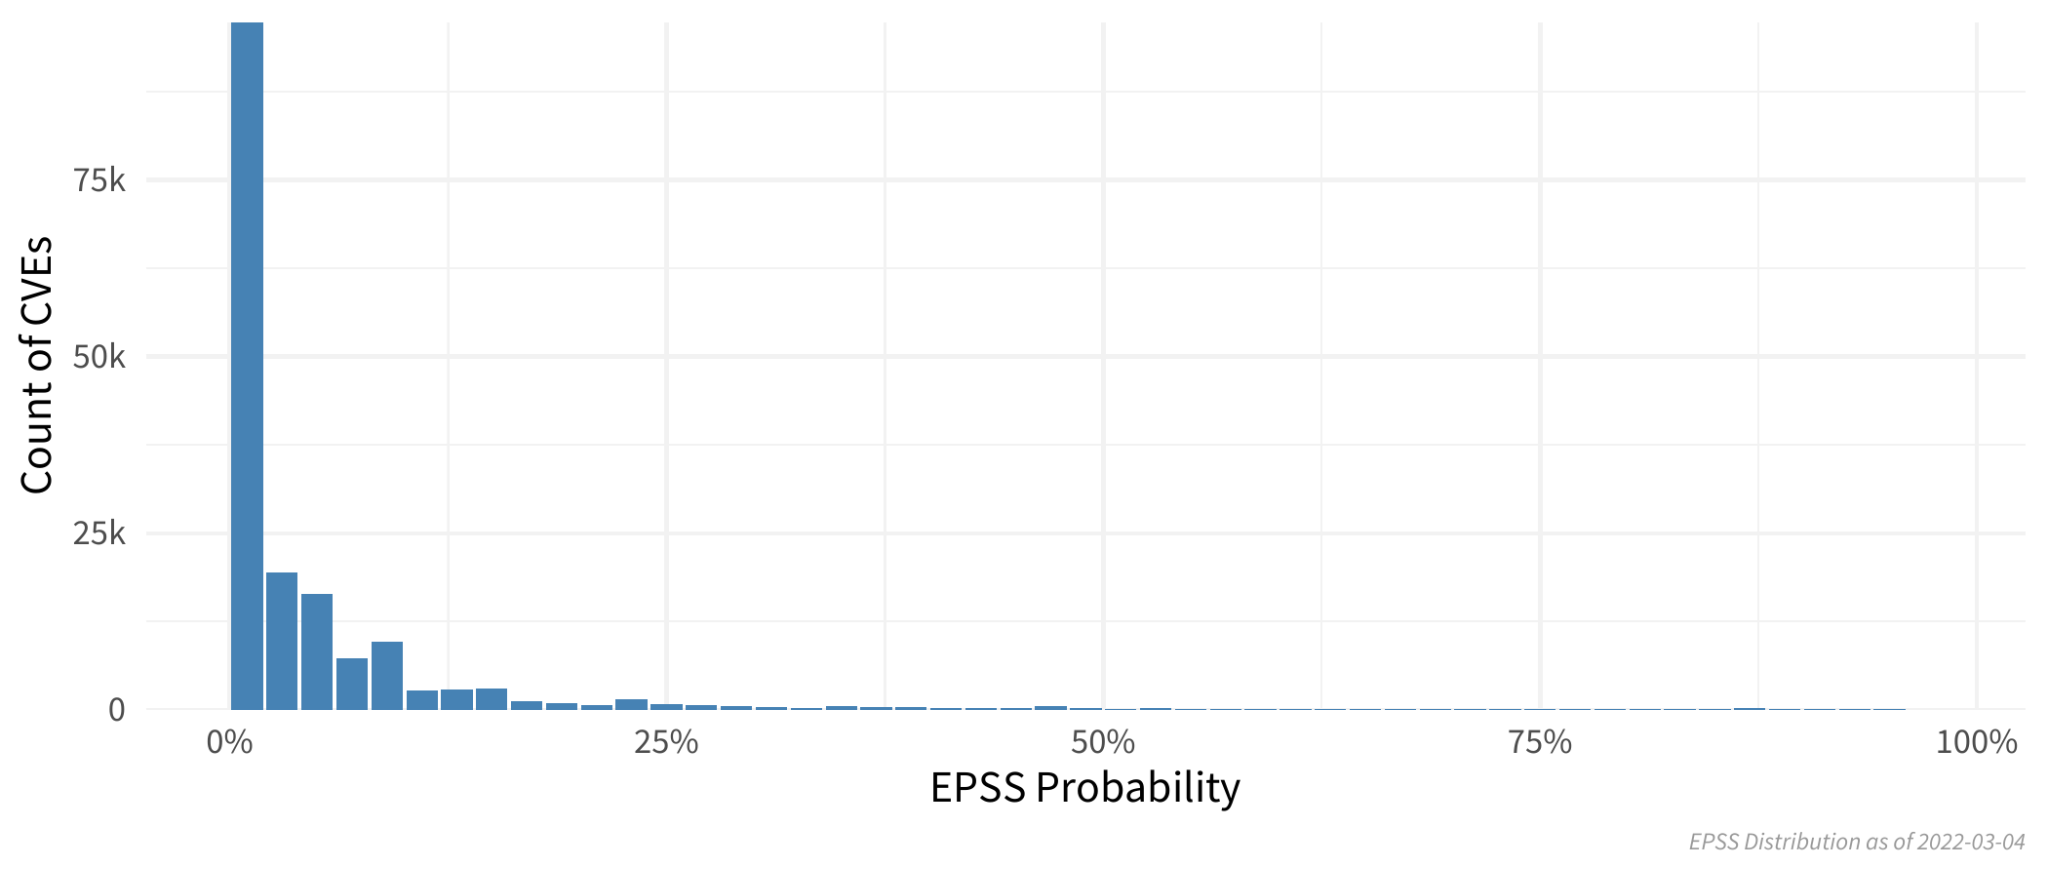
\includegraphics[width=\textwidth]{resources/EPSS_Prob_Dist.png}
    \caption{Distribution of \ac{EPSS} probabilities as of 2022-03-04 \autocite{first_exploit_2022}.}
    \label{fig:epss-distribution}
\end{figure}

The visualized distribution highlights the role of \ac{EPSS} in guiding remediation strategies. By focusing on high-probability vulnerabilities, organizations can efficiently allocate their resources to address the most critical threats, reducing the likelihood of exploitation while maintaining operational security.

Within this thesis, the \texttt{first.org} \ac{EPSS} database is queried via the provided \ac{API} to retrieve exploit probability scores for each identified vulnerability. These scores are integrated into the multidimensional classification model, combining them with \ac{CVSS} technical severity to enhance prioritization accuracy (see section~\ref{sec:algorithm-classifications}).

\subsection{Other Vulnerability Databases}
\label{subsec:other-vulnerability-databases}

While databases such as the \ac{DST}\footnote{\url{https://security-tracker.debian.org/tracker/}} and the \ac{RHD}\footnote{\url{https://access.redhat.com/security/security-updates/cve}} also offer valuable insights for vulnerability management, they are not examined in detail in this thesis due to their limited scope and specific focus on particular software ecosystems. These databases primarily target vulnerabilities within their respective platforms  -  Debian-based and Red Hat systems  -  which can limit their general applicability across a wider range of software environments. The primary focus of this work is on vulnerability databases that provide broader, cross-platform coverage and have higher adoption rates across diverse development ecosystems. As such, databases like the \ac{NVD}, \ac{OSV}, and \ac{GAD} were selected for their comprehensive, ecosystem-agnostic data.

\section{Scientific Foundations of the Expert Questionnaire}
\label{sec:scientific-foundations-questionnaire}

The expert evaluation conducted within this thesis can be understood as a form of self-report methodology, as it depends on subjective judgments provided by experts based on their professional knowledge and experience. According to \textcite{lucas_richard_e_global_2006}, self-report methodologies require respondents to interpret questions, recall relevant information, form judgments, and convert these judgments into responses. These cognitive processes underline the importance of careful questionnaire design, as each step can be substantially influenced by question wording, format, and context, thereby affecting the validity of responses \autocite{lucas_richard_e_global_2006}.

Further, as \textcite{schwarz_self-reports_1999} notes, respondents infer the pragmatic meaning of questions using contextual clues, including explicit framing provided by the questionnaire. Clearly specifying the context of the questionnaire as an expert evaluation conducted within a master's thesis on cybersecurity can thus guide respondents toward relevant and meaningful responses, enhancing the methodological rigor and reliability of the results.

Therefore, careful attention to question wording, context specification, and clear framing is essential for ensuring the validity of the expert evaluation, which this work has explicitly considered in designing the structured questionnaire.

The structured questionnaire used for the evaluation is presented in Appendix~\ref{appendix:questionnaire}.

\section{Lessons Learned from Existing Tools and \\ Their Impact on the Proposed Approach}
\label{sec:lessons-from-tools}

The literature review of current vulnerability management tools (refer to section~\ref{sec:multidimensional-approaches-tools}) shows that leading solutions adopt a multidimensional approach to vulnerability detection, assessment, and remediation. This approach is essential because vulnerabilities vary significantly in their characteristics and impacts, necessitating a comprehensive framework to effectively manage them. The following summary consolidates the scoring factors employed by prominent tools such as Tenable, Rapid7, and Snyk into a concise and comparative overview. By highlighting their respective strengths and specific scoring dimensions, this overview informs the development of a robust, hybrid vulnerability management model.

\subsection*{Consolidated Scoring Factors}
\label{subsec:consolidated_scoring_factors}

\begin{table}[H]
	\centering
	\label{tab:consolidated_scoring_factors}
	\begin{tabular}{|p{3.5cm}|p{3.2cm}|p{3.2cm}|p{3.2cm}|}
		\hline
		\textbf{Scoring Factor}               & \textbf{Tenable}               & \textbf{Rapid7}               & \textbf{Snyk}                   \\ \hline
		Technical Severity (CVSS)             & Yes & Yes & Yes                             \\ \hline
		Exploit Availability \& Maturity      & Yes (VPR)                      & Yes (honeypot data)    & Yes                             \\ \hline
		Threat Intelligence                   & Yes                            & Yes              & No                              \\ \hline
		Business Context \& Asset Criticality & Yes                            & Yes                           & No                              \\ \hline
		Exposure                              & No                             & Yes                           & No                              \\ \hline
		Fix Availability \& Vulnerability Age & Yes (vulnerability age) & No                            & Yes (patch availability) \\ \hline
		Additional Data Sources               & Yes (internal DB)       & Yes (partner data)     & Yes (public/internal DB) \\ \hline
	\end{tabular}
    	\caption{Consolidated Scoring Factors used by Tenable, Rapid7, and Snyk}
\end{table}

\subsection*{Summary and Impact on the Proposed Approach}
\label{subsec:summary_impact}

Insights from Tenable, Rapid7, and Snyk highlight the need for a multidimensional approach to vulnerability management that integrates technical severity with real-world exploit likelihood. A notable limitation of relying solely on \ac{CVSS} is scoring inconsistency, which can cause misaligned remediation priorities \autocite{spring_time_2021}.

Integrating the quantitative severity assessment provided by \ac{CVSS} with the probabilistic predictions from \ac{EPSS} into a unified scoring system addresses this issue. This hybrid model incorporates factors such as vendor intelligence, vulnerability age, exploit availability, exploit maturity, and threat intelligence, which are dimensions successfully utilized by Tenable, Rapid7, and Snyk (see section~\ref{subsec:consolidated_scoring_factors}). The studies conducted by \textcite{jacobs_exploit_2021} and \textcite{first_epss_2021} confirm that incorporating threat-likelihood metrics alongside \ac{CVSS} improves remediation efficiency by reducing patch workloads while effectively mitigating actively exploited vulnerabilities.

Using \ac{EPSS} and \ac{CVSS} together significantly enhances prioritization: \ac{CVSS} quantifies the \emph{impact} of vulnerabilities, while \ac{EPSS} estimates their \emph{likelihood of exploitation} based on empirical data.

Figure~\ref{fig:epss_cvss_compare} illustrates this concept clearly, showing the relationship between \ac{EPSS} probabilities and \ac{CVSS} scores for vulnerabilities as of 2021-05-16.

\begin{figure}[H]
	\centering
	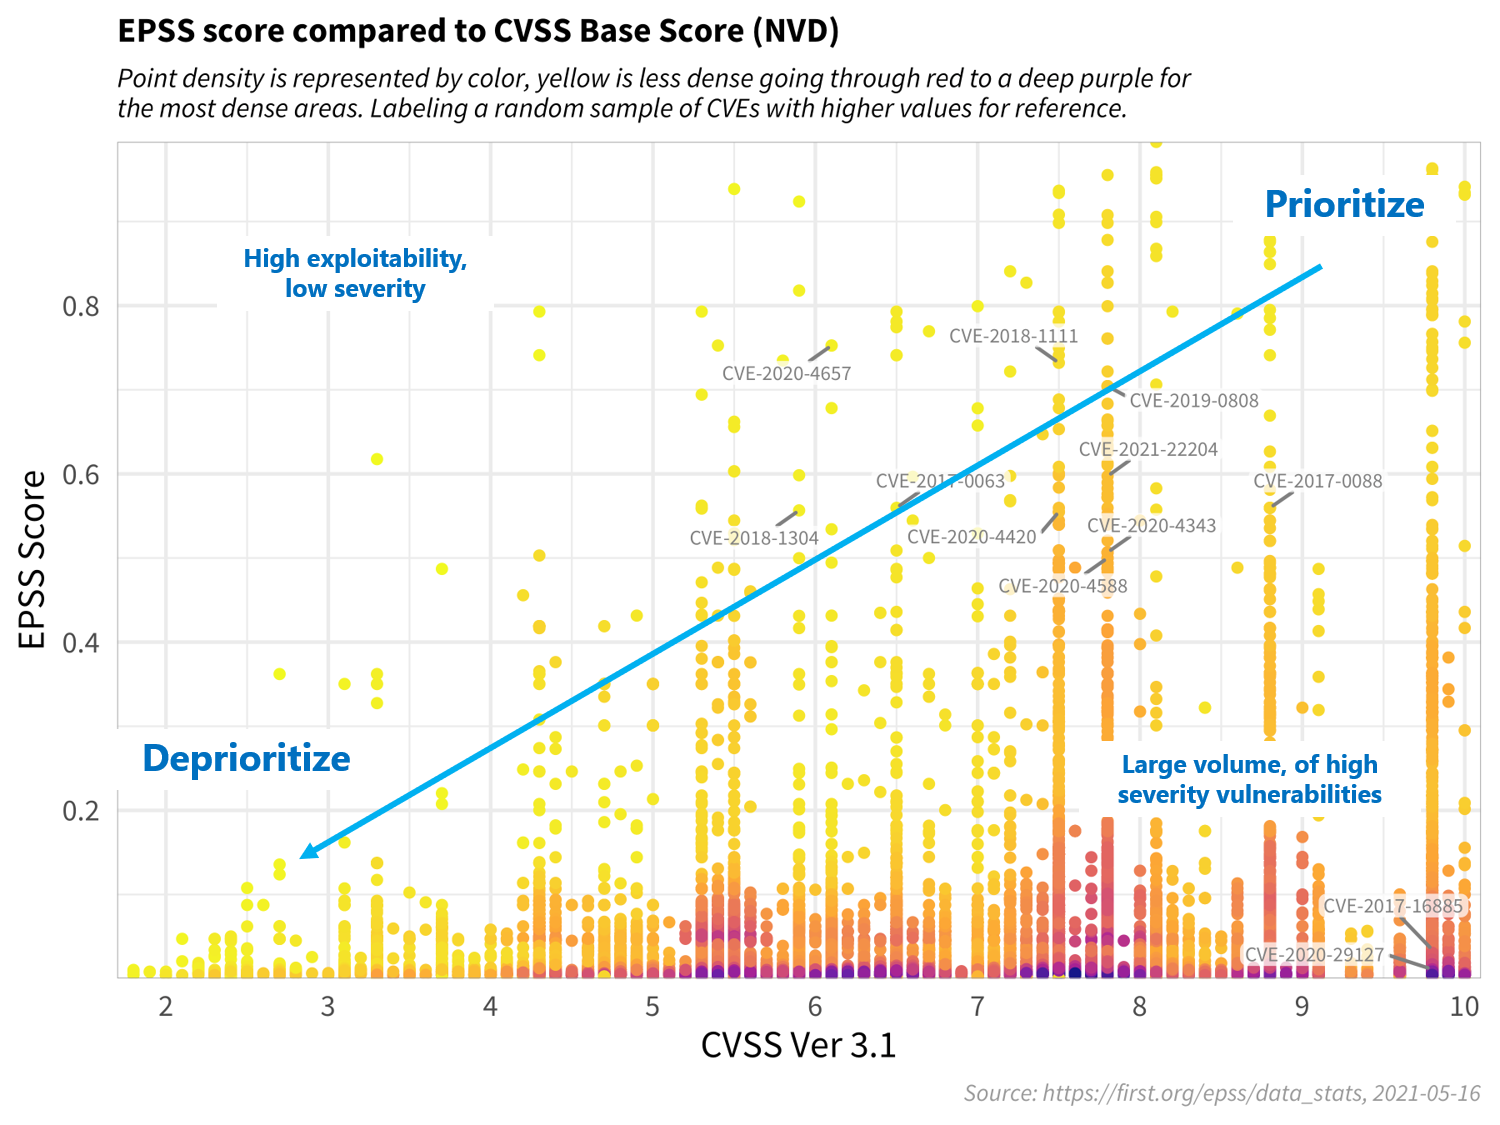
\includegraphics[scale=0.46]{resources/EPSS_CVSS_Compare.png}
	\caption[\ac{EPSS} and \ac{CVSS} Comparison]{Illustration of how \ac{EPSS} probabilities and \ac{CVSS} severity scores complement each other for better risk-based prioritization \autocite{first_epss_2021}.}
	\label{fig:epss_cvss_compare}
\end{figure}

Most vulnerabilities cluster towards lower exploit probabilities. Only a small fraction of vulnerabilities have \ac{EPSS} scores above 0.5. Although there is some correlation between \ac{EPSS} and \ac{CVSS} scores, this visualization clearly indicates that attackers do not exclusively target vulnerabilities that produce the greatest impact or are necessarily the easiest to exploit.

For prioritization, vulnerabilities in the lower-left quadrant (low probability, low impact) can typically be deprioritized. Vulnerabilities in the upper-left quadrant (high exploit probability, low impact) should be evaluated further, particularly in chained attack scenarios. Those in the lower-right quadrant (low exploit probability, high impact) warrant monitoring due to potential future exploitability. Vulnerabilities in the upper-right quadrant represent the highest risks (high probability, high impact) and must be addressed first \autocite{first_epss_2021}.

After establishing this combined severity score, the thesis applies a decision tree for remediation planning, drawing on the \ac{SSVC} framework (see section \ref{subsec:stakeholder-specific-vulnerability}). This tree incorporates \emph{Vulnerability Classification}, \emph{Patch Availability}, \emph{System Usage} (public or internal), \emph{Asset Criticality}, \emph{Fix Complexity}, \emph{Personal Code Ownership}, \emph{Exploit Likelihood}, \emph{Observed Exploits}, \emph{Compliance Requirement}, and \emph{Business Impact}. The required input data for these parameters is collected through a user query in the frontend, ensuring that context-specific factors are considered in the decision-making process. 

By blending a robust quantitative metric with a well-defined remediation process, the proposed framework addresses all of the key data considerations employed by Tenable, Rapid7, and Snyk - ensuring precise prioritization and more informed remediation strategies for critical vulnerabilities.